\documentclass[11pt,a4paper]{article}

\usepackage[utf8]{inputenc}
\usepackage[T1]{fontenc}
\usepackage[margin=2.4cm,top=2.6cm,bottom=2.4cm]{geometry}
\usepackage{lmodern}
\usepackage{microtype}
\usepackage{booktabs}
\usepackage{array}
\usepackage{enumitem}
\usepackage{listings}
\usepackage{xcolor}
\usepackage{titlesec}
\usepackage{fancyhdr}
\usepackage{tcolorbox}
\usepackage{tikz}
\usetikzlibrary{positioning,arrows,calc,fit,backgrounds}
\usepackage[colorlinks=true,linkcolor=accent,urlcolor=accent,citecolor=accent]{hyperref}

% ---------------------------------------------------------------- palette ----
\definecolor{accent}{HTML}{4F46E5}
\definecolor{ink}{HTML}{18181B}
\definecolor{muted}{HTML}{71717A}
\definecolor{hairline}{HTML}{E4E4E7}
\definecolor{surface}{HTML}{FAFAFA}
\definecolor{warnbg}{HTML}{FFFBEB}
\definecolor{warnline}{HTML}{D97706}
\definecolor{okline}{HTML}{059669}

\color{ink}

% ------------------------------------------------------------- structure ----
\titleformat{\section}{\large\bfseries\color{accent}}{\thesection}{0.6em}{}
\titleformat{\subsection}{\normalsize\bfseries\color{ink}}{\thesubsection}{0.6em}{}
\titlespacing*{\section}{0pt}{1.4em}{0.5em}
\titlespacing*{\subsection}{0pt}{1.0em}{0.35em}

\pagestyle{fancy}
\fancyhf{}
\renewcommand{\headrulewidth}{0.4pt}
\renewcommand{\headrule}{\color{hairline}\hrule height\headrulewidth}
\fancyhead[L]{\footnotesize\color{muted}Real-time speech-to-text — integration contract}
\fancyhead[R]{\footnotesize\color{muted}\thepage}

% ----------------------------------------------------------------- code ----
\lstdefinestyle{docie}{
  basicstyle=\ttfamily\small,
  backgroundcolor=\color{surface},
  frame=single,
  rulecolor=\color{hairline},
  framesep=6pt,
  xleftmargin=2pt,
  xrightmargin=2pt,
  breaklines=true,
  columns=fullflexible,
  keepspaces=true,
  showstringspaces=false,
  stringstyle=\color{accent},
  commentstyle=\color{muted}\itshape,
  aboveskip=0.9em,
  belowskip=0.9em,
}
\lstset{style=docie}

% ------------------------------------------------------------ tikz style ----
\tikzset{
  lane/.style={draw=hairline, fill=white, rounded corners=3pt, line width=0.7pt,
               minimum width=3.3cm, minimum height=0.95cm, align=center,
               font=\small\bfseries},
  life/.style={draw=hairline, dashed, line width=0.7pt},
  msg/.style={->, >=latex, line width=0.8pt, draw=accent, font=\scriptsize},
  msgback/.style={->, >=latex, line width=0.8pt, draw=muted, font=\scriptsize, dashed},
  audio/.style={->, >=latex, line width=1.6pt, draw=accent, font=\scriptsize},
  stepnum/.style={circle, fill=accent, text=white, font=\scriptsize\bfseries,
               inner sep=1.4pt, minimum size=3.6mm},
  box/.style={draw=hairline, fill=white, rounded corners=3pt, line width=0.7pt,
              minimum height=1.05cm, align=center, font=\small},
  note/.style={font=\scriptsize\itshape, text=muted, align=center},
}

% --------------------------------------------------------------- boxes ----
\newtcolorbox{statusbox}{
  colback=warnbg, colframe=warnline, boxrule=0.8pt, arc=3pt,
  left=10pt, right=10pt, top=8pt, bottom=8pt,
}
\newtcolorbox{dontbox}[1]{
  colback=white, colframe=warnline, boxrule=1.2pt, arc=3pt,
  left=10pt, right=10pt, top=8pt, bottom=8pt,
  title={\bfseries #1}, coltitle=white, colbacktitle=warnline,
  fonttitle=\normalsize,
}
\newtcolorbox{askbox}{
  colback=white, colframe=accent, boxrule=1pt, arc=3pt,
  left=10pt, right=10pt, top=8pt, bottom=8pt,
}

\setlist[itemize]{leftmargin=1.3em, itemsep=0.32em, topsep=0.35em}
\setlist[enumerate]{leftmargin=1.5em, itemsep=0.45em, topsep=0.35em}

\begin{document}
\thispagestyle{empty}

% ----------------------------------------------------------- title block ----
\begin{flushleft}
{\color{accent}\rule{\textwidth}{2.2pt}}\\[1.1em]
{\Huge\bfseries Real-time speech-to-text}\\[0.45em]
{\Large\color{muted} Integration contract}\\[1.1em]
{\color{hairline}\rule{\textwidth}{0.6pt}}\\[0.7em]
{\small\color{muted}
DocIE inference platform \quad$\longleftrightarrow$\quad Cynov ERP \hfill \today}
\end{flushleft}

\vspace{1.3em}

\begin{statusbox}
\textbf{Status: proposal for review. Not yet implemented.}\par\smallskip
This document exists so both teams agree the contract \emph{before} either side builds
against it. Endpoint paths, field names and message types may still change in response
to your feedback. Please do not begin implementation until we have both signed off on
Section~\ref{sec:erp}.
\end{statusbox}

\vspace{0.6em}

\section{What we are building}

The ERP captures microphone audio in the browser and displays a live transcript as the
user speaks. Audio travels to the DocIE inference platform over a WebSocket; partial
transcripts return within roughly one second, and a stable final transcript is emitted
each time the speaker pauses.

The model is French-capable (fr-FR and fr-CA) and natively streaming, so transcription is
incremental rather than \emph{upload a file and wait}. File-based transcription is
explicitly outside the scope of this work.

\vspace{0.8em}
\begin{center}
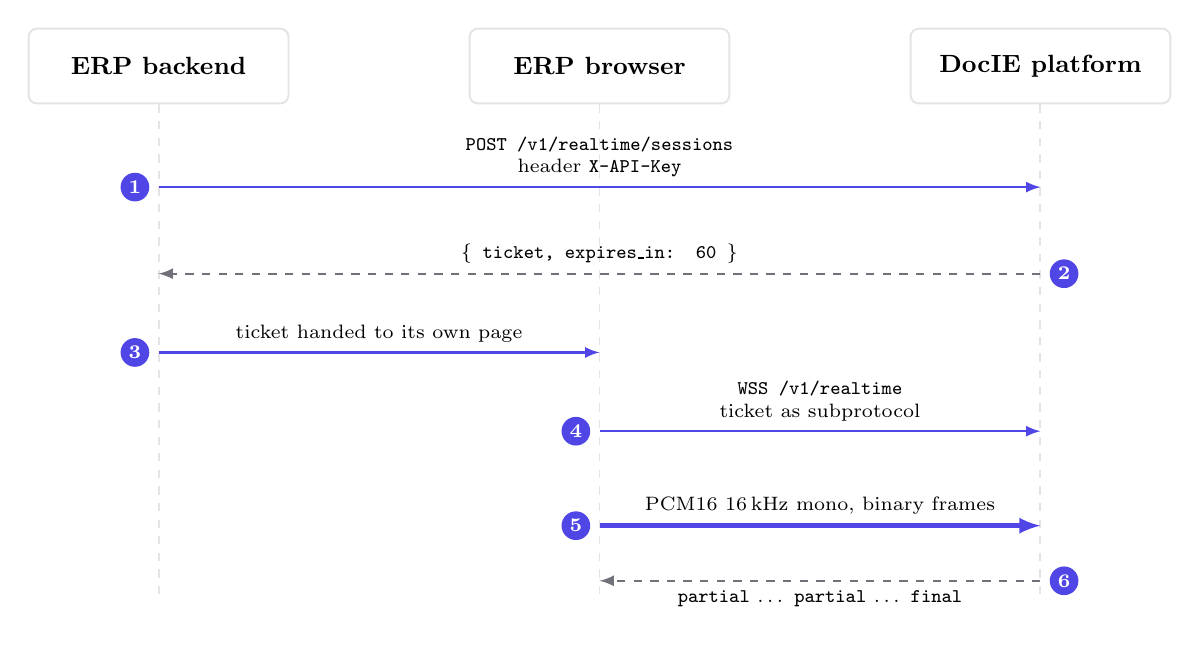
\begin{tikzpicture}[node distance=0pt]

  % lanes
  \node[lane] (be)  at (0,0)     {ERP backend};
  \node[lane] (br)  at (5.6,0)   {ERP browser};
  \node[lane] (dc)  at (11.2,0)  {DocIE platform};

  % lifelines
  \draw[life] (be.south)  -- ++(0,-6.25);
  \draw[life] (br.south)  -- ++(0,-6.25);
  \draw[life] (dc.south)  -- ++(0,-6.25);

  % 1 mint
  \draw[msg] ([yshift=-1.05cm]be.south) -- node[above,midway,align=center]
       {\texttt{POST /v1/realtime/sessions}\\ header \texttt{X-API-Key}}
       ([yshift=-1.05cm]dc.south);
  \node[stepnum] at ([xshift=-3mm,yshift=-1.05cm]be.south) {1};

  % 2 ticket back
  \draw[msgback] ([yshift=-2.15cm]dc.south) -- node[above,midway]
       {\texttt{\{ ticket, expires\_in: 60 \}}}
       ([yshift=-2.15cm]be.south);
  \node[stepnum] at ([xshift=3mm,yshift=-2.15cm]dc.south) {2};

  % 3 hand to browser
  \draw[msg] ([yshift=-3.15cm]be.south) -- node[above,midway]
       {ticket handed to its own page}
       ([yshift=-3.15cm]br.south);
  \node[stepnum] at ([xshift=-3mm,yshift=-3.15cm]be.south) {3};

  % 4 open socket
  \draw[msg] ([yshift=-4.15cm]br.south) -- node[above,midway,align=center]
       {\texttt{WSS /v1/realtime}\\ ticket as subprotocol}
       ([yshift=-4.15cm]dc.south);
  \node[stepnum] at ([xshift=-3mm,yshift=-4.15cm]br.south) {4};

  % 5 audio up
  \draw[audio] ([yshift=-5.35cm]br.south) -- node[above,midway]
       {PCM16 16\,kHz mono, binary frames}
       ([yshift=-5.35cm]dc.south);
  \node[stepnum] at ([xshift=-3mm,yshift=-5.35cm]br.south) {5};

  % 6 transcripts down
  \draw[msgback] ([yshift=-6.05cm]dc.south) -- node[below,midway]
       {\texttt{partial} \ldots\ \texttt{partial} \ldots\ \texttt{final}}
       ([yshift=-6.05cm]br.south);
  \node[stepnum] at ([xshift=3mm,yshift=-6.05cm]dc.south) {6};

\end{tikzpicture}

\vspace{0.3em}
{\scriptsize\color{muted} Steps 1--3 are server-to-server and happen once per dictation
session. Only the thick arrow carries audio.}
\end{center}

\section{The one thing that must not happen}

\begin{dontbox}{Never send a DocIE API key to the browser}
API keys on our platform are long-lived and unscoped: one key grants access to every
model on the \texttt{/v1} API, and all usage is billed and audited against it. A key
embedded in ERP frontend JavaScript is readable by every ERP user and by anything else
running in that page.\par\smallskip
Treat it exactly as you would a database password.
\end{dontbox}

This is not a restriction we can configure away, and it is the reason the flow has two
steps instead of one. A browser is not a place a durable credential can live, so the
browser is given a short-lived ticket instead. The API key never leaves your server.

\section{What the ERP team implements}
\label{sec:erp}

Two pieces of work, one on each side of your stack.

\subsection{Backend: mint a ticket (server-to-server)}

Your backend already holds the DocIE API key. When a user opens the dictation UI, your
backend requests a ticket and returns it to that user's page.

\begin{lstlisting}
curl -X POST https://api.inference.cynov.com/v1/realtime/sessions \
  -H "X-API-Key: $DOCIE_API_KEY" \
  -H "Content-Type: application/json" \
  -d '{"language": "fr"}'
\end{lstlisting}

\begin{lstlisting}
{
  "ticket":     "docie_rt_<opaque>",
  "expires_in": 60,
  "ws_url":     "wss://api.inference.cynov.com/v1/realtime"
}
\end{lstlisting}

\noindent Properties of the ticket, which shape how you use it:

\begin{center}
\renewcommand{\arraystretch}{1.35}
\begin{tabular}{@{}>{\bfseries}p{3.1cm}p{11.2cm}@{}}
\toprule
Short-lived    & About 60 seconds --- enough to open the socket, not enough to be worth
                 storing. Mint one when the user presses record. \\
Single-use     & Consumed by the first socket that presents it; a second connection with
                 the same ticket is refused. \\
Narrowly scoped & Opens a transcription socket and authorises nothing else. It is not a
                 substitute for the API key. \\
Attributed     & All usage is recorded against the API key that minted it, so your
                 reporting stays per-key however many users dictate. \\
\bottomrule
\end{tabular}
\end{center}

\noindent Do not cache tickets or share one between users. Minting is cheap.

\subsection{Browser: open the socket and stream audio}

\begin{lstlisting}
const ws = new WebSocket(ws_url, [ticket]);   // ticket as subprotocol
ws.binaryType = "arraybuffer";
\end{lstlisting}

The ticket travels as a WebSocket subprotocol (\texttt{Sec-WebSocket-Protocol}), the only
header a browser is able to set on a WebSocket handshake. We deliberately keep it out of
the query string, because URLs end up in proxy logs, access logs and browser history. If
your stack cannot set a subprotocol, tell us and we will enable a query-parameter
fallback --- but the subprotocol is preferred.

\vspace{0.9em}
\begin{center}
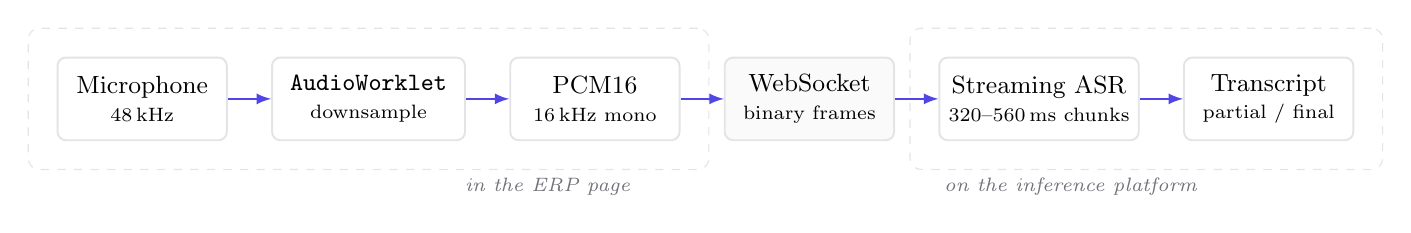
\begin{tikzpicture}[node distance=5.5mm]

  \node[box, minimum width=2.15cm] (mic)  {Microphone\\[-1pt]{\scriptsize 48\,kHz}};
  \node[box, minimum width=2.45cm, right=of mic] (work) {\texttt{AudioWorklet}\\[-1pt]{\scriptsize downsample}};
  \node[box, minimum width=2.15cm, right=of work] (pcm)  {PCM16\\[-1pt]{\scriptsize 16\,kHz mono}};
  \node[box, minimum width=2.15cm, right=of pcm, fill=surface] (ws)   {WebSocket\\[-1pt]{\scriptsize binary frames}};
  \node[box, minimum width=2.45cm, right=of ws] (asr)  {Streaming ASR\\[-1pt]{\scriptsize 320--560\,ms chunks}};
  \node[box, minimum width=2.15cm, right=of asr] (out)  {Transcript\\[-1pt]{\scriptsize partial / final}};

  \foreach \a/\b in {mic/work, work/pcm, pcm/ws, ws/asr, asr/out}
    \draw[->, >=latex, line width=0.8pt, draw=accent] (\a) -- (\b);

  \node[note, below=3.5mm of pcm, xshift=-6mm] {in the ERP page};
  \node[note, below=3.5mm of asr, xshift=4mm] {on the inference platform};

  \begin{scope}[on background layer]
    \node[draw=hairline, dashed, rounded corners=4pt, inner sep=3.6mm,
          fit=(mic)(pcm)] {};
    \node[draw=hairline, dashed, rounded corners=4pt, inner sep=3.6mm,
          fit=(asr)(out)] {};
  \end{scope}

\end{tikzpicture}
\end{center}

\subsubsection*{Audio format}

\begin{center}
\renewcommand{\arraystretch}{1.25}
\begin{tabular}{@{}>{\bfseries}ll@{}}
\toprule
Encoding    & 16-bit signed PCM, little-endian \\
Sample rate & 16\,000 Hz \\
Channels    & 1 (mono) \\
Frame size  & 20--100\,ms per message (320--1600 samples) \\
Transport   & binary WebSocket frames \\
\bottomrule
\end{tabular}
\end{center}

Browsers capture at 44.1 or 48\,kHz, so the page must downsample to 16\,kHz. Use an
\texttt{AudioWorklet} rather than the deprecated \texttt{ScriptProcessorNode}: it runs off
the main thread and will not glitch when the ERP interface is busy. Resampling in the
browser also keeps that work off our shared inference hosts, which directly raises how
many simultaneous speakers we can serve.

Please do not send WebM, Opus or MP3. The runtime consumes raw PCM; a container format
would have to be decoded server-side and would add latency.

\subsubsection*{Messages you will receive}

Text frames, one JSON object each.

\begin{lstlisting}
{ "type": "partial", "text": "bonjour je voudrais commander" }
\end{lstlisting}

\begin{lstlisting}
{ "type":  "final",
  "text":  "Bonjour, je voudrais commander trois cartons.",
  "start": 0.42,
  "end":   3.87 }
\end{lstlisting}

\begin{lstlisting}
{ "type": "error", "code": "ticket_expired", "message": "..." }
\end{lstlisting}

Render \texttt{partial} as provisional text --- greyed or italic, your choice --- and
replace it when the matching \texttt{final} arrives. Several partials per second are
normal and each supersedes the previous one. A \texttt{final} is stable and will not be
revised; only finals should be persisted. The socket closes after an \texttt{error}.

\subsubsection*{Ending a session}

Send a text frame \texttt{\{"type": "close"\}} when the user stops dictating, then close
the socket. We flush any audio still in flight and emit one last \texttt{final} before
closing. Dropping the connection also works, but may lose the trailing phrase.

\section{What we need from you}

\begin{askbox}
\begin{enumerate}
  \item \textbf{The exact browser origin(s)} that will open sockets, for example
        \texttt{https://newapp.cynov.com}. WebSockets are not subject to the same-origin
        policy, so we validate the \texttt{Origin} header against an allowlist during the
        handshake. Without this, a stolen ticket would work from any website.
  \item \textbf{Expected concurrency} --- how many users might dictate simultaneously at
        peak. This is our real capacity constraint: cost scales with the number of live
        speakers, and the inference hosts are CPU-only and shared with other workloads. We
        will cap concurrent sockets per API key, and we would rather agree that number
        with you than discover it.
  \item \textbf{Where the transcript needs to land.} If only the browser needs it --- the
        user reads it and saves a form --- the flow above is complete. If your
        \emph{backend} needs the text, to file it into a record, please say so now:
        relaying it from the browser back up to your server is lossy and racy, and we
        would instead deliver finals to a webhook you expose, or have your backend hold
        the socket.
  \item \textbf{A sample of representative French audio}, if you can share one. Published
        accuracy figures for these models are measured on read speech. Spontaneous
        business French, with crosstalk, accents and background noise, behaves very
        differently, and we would rather measure on your real input than on a benchmark.
\end{enumerate}
\end{askbox}

\section{Open points on our side}

Listed for transparency. None of them change what Section~\ref{sec:erp} asks of you.

\begin{itemize}
  \item \textbf{Latency.} The model exposes chunk sizes of 80, 160, 320, 560 and
        1120\,ms. We expect to ship 320 or 560\,ms, which keeps end-to-end latency under
        a second. Smaller chunks feel more immediate and cost some accuracy.
  \item \textbf{Throughput on CPU.} Our fleet has no GPUs. We are measuring the real-time
        factor on the actual hardware before committing, because the model's published
        benchmarks are GPU-only. This is the main risk to the schedule, and it determines
        the answer to ask~2 above.
  \item \textbf{Metering.} Streaming is accounted in audio seconds rather than requests.
        Our per-key usage reporting is being extended accordingly.
\end{itemize}

\section{Summary of the contract}

\begin{center}
\renewcommand{\arraystretch}{1.45}
\begin{tabular}{@{}p{7.1cm}p{7.1cm}@{}}
\toprule
{\color{accent}\bfseries ERP team} & {\color{accent}\bfseries Inference platform} \\
\midrule
Hold the API key server-side only &
Mint short-lived, single-use, streaming-scoped tickets \\
Mint one ticket per dictation session &
Validate the ticket and the \texttt{Origin} on handshake \\
Capture microphone audio, downsample to 16\,kHz mono PCM16 &
Transcribe incrementally, stream partials and finals \\
Render partials, persist only finals &
Attribute all usage to the minting API key \\
Provide origin(s), expected concurrency, sample audio &
Cap concurrent sockets per key, publish the final contract \\
\bottomrule
\end{tabular}
\end{center}

\vspace{1.1em}
\noindent
If anything here does not fit how the ERP is built, please say so now rather than after
it is implemented. The shape of the authentication flow is fixed by the
browser-credential constraint in Section~2; almost everything else is negotiable.

\end{document}
